\documentclass[letterpaper, 11pt]{article}
\usepackage[utf8]{inputenc}
\usepackage{mathptmx}
\usepackage{natbib}
\usepackage[top=1in, bottom=1.25in, left=1.25in, right=1.25in]{geometry}
\usepackage{enumitem}
\usepackage[usenames,dvipsnames]{xcolor}
\usepackage{hyperref}
\hypersetup{colorlinks=true,allcolors=MidnightBlue}
\usepackage{titlesec}
\usepackage{graphicx}
\usepackage{wrapfig}
\usepackage{enumitem}
\usepackage{array}
\usepackage{booktabs}
%%%%%%%%%%%%%%%
%% FEEL FREE TO ADD MORE PACKAGES %%% 
%%%%%%
%%% LaTeX 
%% https://www.overleaf.com/learn/latex/Learn_LaTeX_in_30_minutes
%% https://www.overleaf.com/learn/latex/Positioning_images_and_tables 

%%% TODO: change TOPIC to your title
\title{CS447 Literature Review: TOPIC}
%%% TODO: change YOURNAME and yournetid to your name and NetId
\author{YOUR NAME,\\ yournetid@illinois.edu}

\begin{document}

\maketitle

\begin{abstract}
The abstract should be a succinct statement of what your review is about. No need to go into details about the individual papers here. 
\end{abstract}

\section{Introduction}
\label{sec:introduction}
The Introduction should explain the topic and research question (if you have one) for your review. Try to motivate your topic/question: why would somebody care about this topic and question? 

\section{Background}
\label{sec:background}
The background section is optional, but if you need to provide more background for readers to understand your review, this is a good place for it. 


\section{Transformers}
\label{sec:transformers} 
You probably want to include one section for each paper that you discuss (feel free to add more subsections and paragraphs as you see fit). 

Provide enough details that your review is self-explanatory (so that your reader doesn't have to consult the original paper to follow your review). But don't just copy from the original paper (except formulas and definitions). 

You should also try to add some analysis, interpretation or critique of your own to the description of each paper (e.g. why is this important? what is the main contribution of this paper? do you see any flaws, open questions, possibilities to build on what was done here?

\paragraph{Citation styles}
Use \texttt{$\backslash$citep} for parenthetical citations, and  \texttt{$\backslash$citet} otherwise, e.g.:\hfill\\ 
``\citet{merrill-etal-2020-formal} define a formal hierarchy of RNN architectures, including Transformers \citep{NIPS2017_3f5ee243}."

\paragraph{Figures, Tables, References}
You can refer to any section, subsection or subsubsection (if you must) of your paper if you add a label below it, e.g. Section~\ref{sec:transformers} doesn't actually talk about transformers, despite its title. 
You can also refer to tables and figures (in fact, don't include tables or figures without referring to them in the body of your paper).

Table~\ref{tab:my_label} is completely made up, but shows you how to include a table. 
Figure~\ref{fig:hal} shows a replica of HAL 9000 at the Carnegie Science Center. 
You're unlikely to need to include actual photographs, but this just shows you how to include figures. 

\section{A Section to teach you a bit of \LaTeX}
\label{sec:section}

\subsection{A subsection to teach you a bit of \LaTeX}
\label{sec:subsection} 




\begin{table}[b] %% use b,t,h
    \centering
    % you can use l,r,c for left-aligned, right-aligned or centered columns
    \begin{tabular}{lrr}
    \toprule
       Model  & BLEU & \# parameters \\ % use ampersands to separate columns and \\ for end of rows
         \midrule
Model A  &  99.5 &  \\ 
Model B & 99.7 & \\
         \bottomrule
    \end{tabular}
    \caption{A completely made-up example table}
    \label{tab:my_label}
\end{table}

\begin{figure}[b]
    \centering
    %%% you should be able to include other image files in the same way
    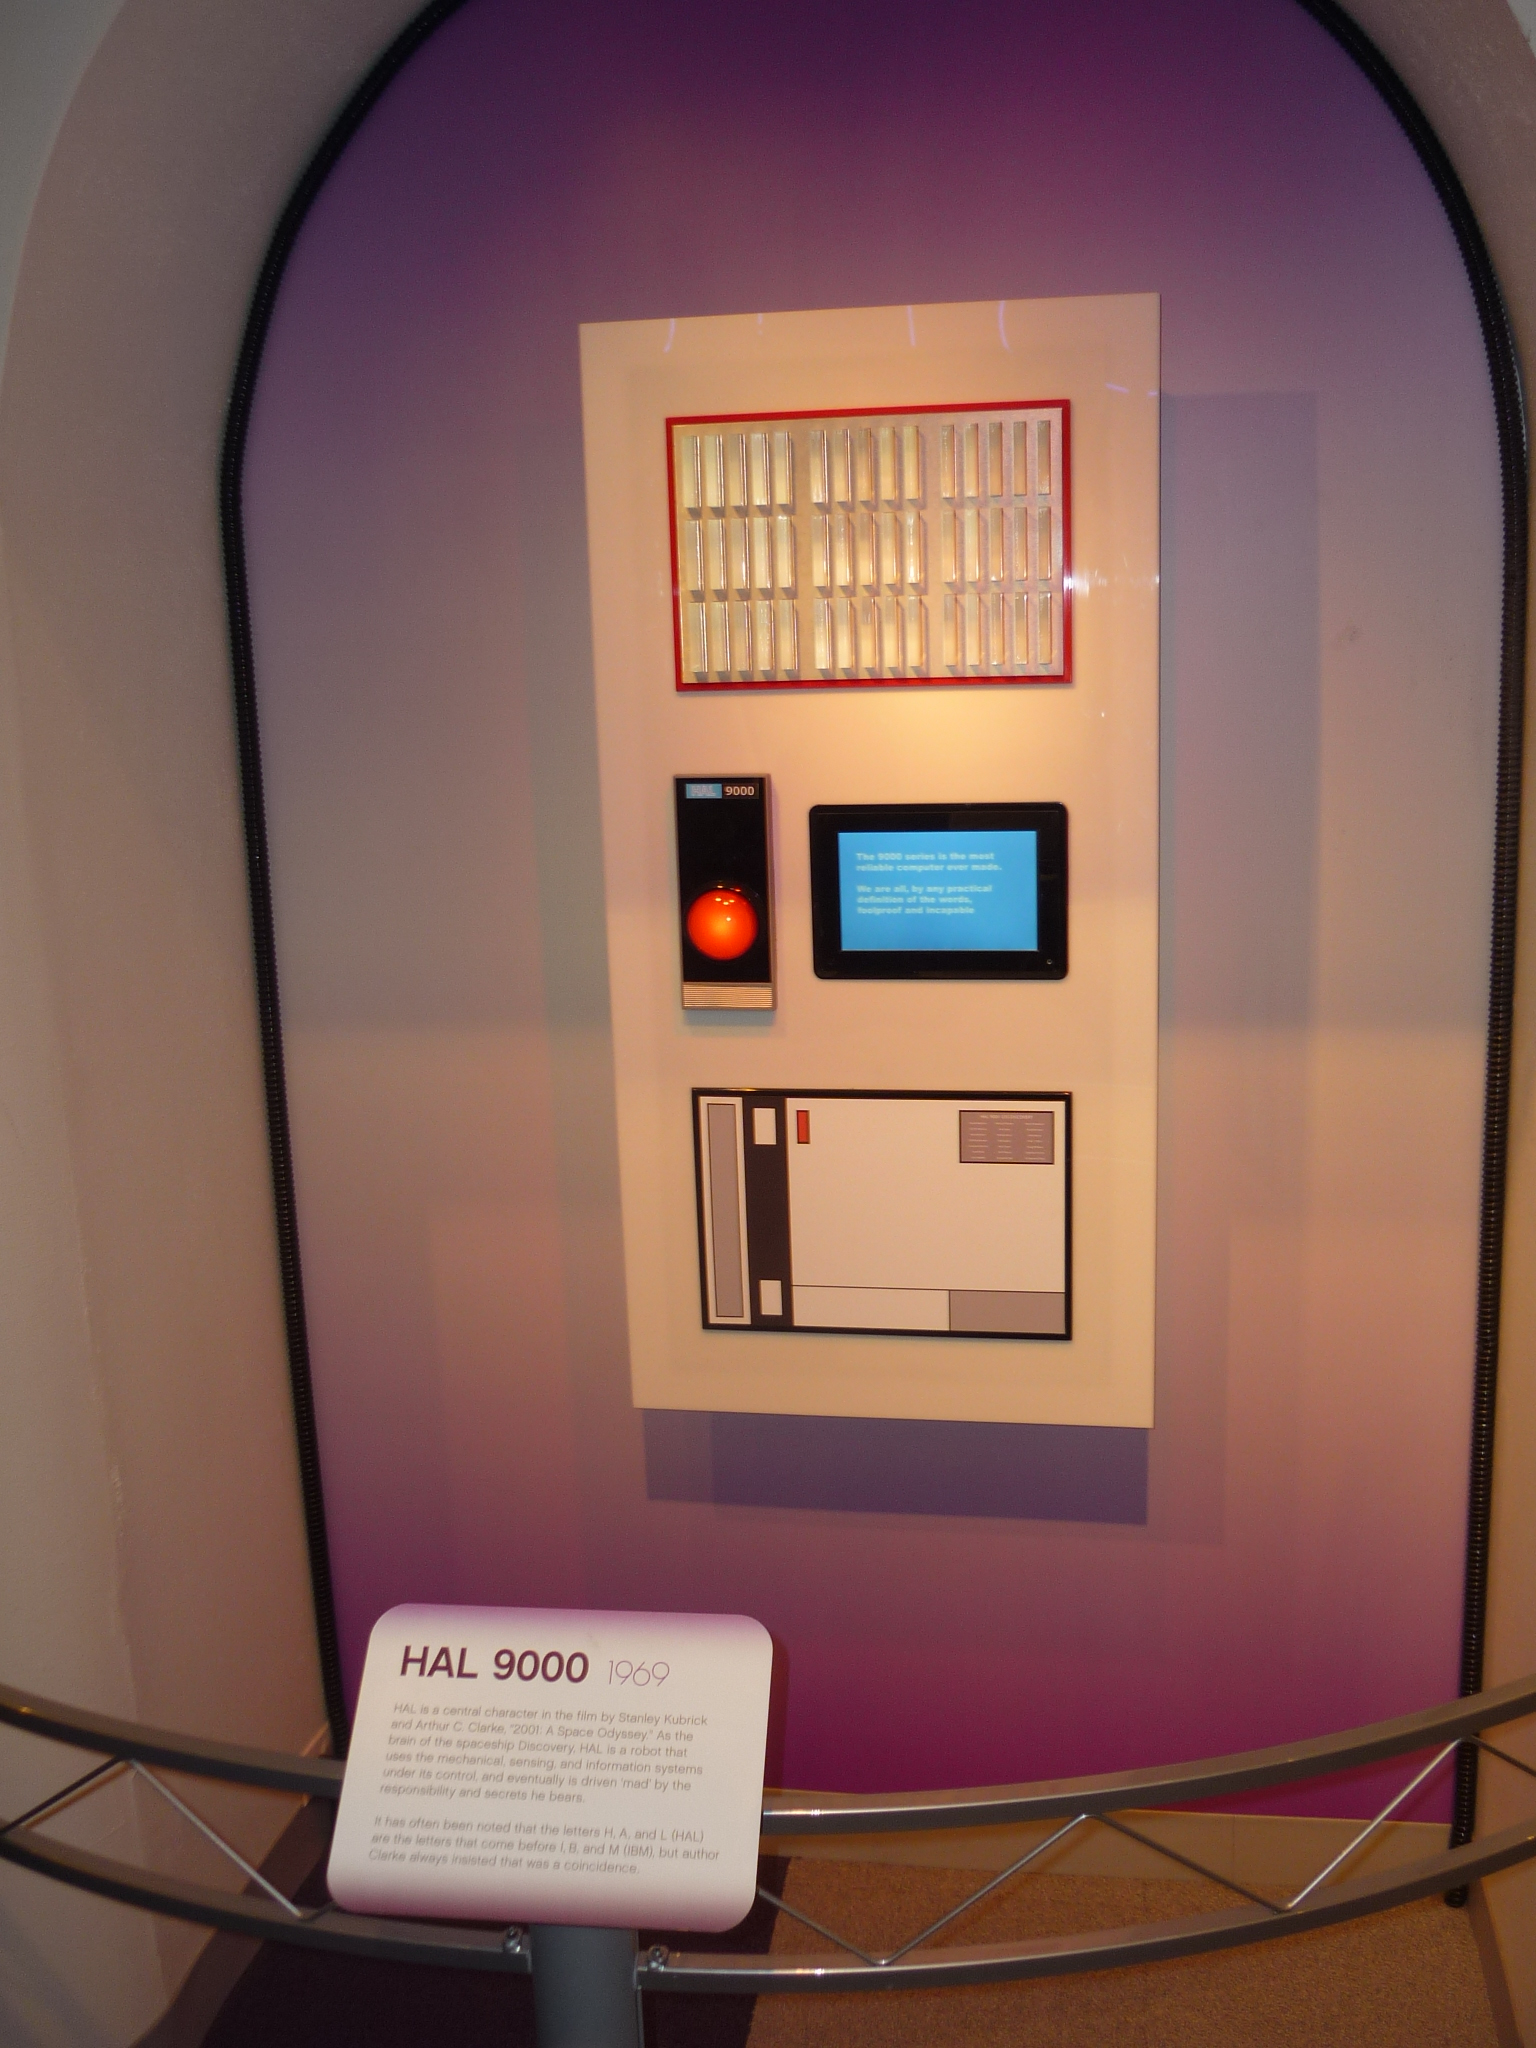
\includegraphics[width=.25\textwidth]{HAL_9000.JPG}
    \caption{A replica of HAL 9000 (from \url{https://en.wikipedia.org/wiki/HAL_9000})}
    \label{fig:hal}
\end{figure}
\section{Discussion}
\label{sec:discussion}
After you have described all of the papers individually, you can now return to your overarching question and synthesize what you have found in these papers to see how well you can answer this question (and discuss if any new questions arise, perhaps). 
You might want to do this in a separate discussion section. Or you can work the discussion into the conclusion. Your choice! 

\section{Conclusion}
\label{sec:conclusion}
Like Sections~\ref{sec:introduction}, \ref{sec:section} and in particular \ref{sec:subsection}, this conclusion doesn't actually say anything, but is just intended to show you how to refer to other sections in your paper. 

Your actual conclusion should restate your question/topic, and summarize the main conclusions you have drawn from the papers you have read. 

\bibliographystyle{acl_natbib}
\bibliography{main}
\end{document}
